\documentclass[problem]{mcs}

\begin{pcomments}
  \pcomment{PS_red_black_card_strategy}
  \pcomment{F16, ps11}
  \pcomment{revised by ARM 12/17/16}
\end{pcomments}

\pkeywords{
  probability
  total_probability
  strategy
  induction
  shuffle
}

%%%%%%%%%%%%%%%%%%%%%%%%%%%%%%%%%%%%%%%%%%%%%%%%%%%%%%%%%%%%%%%%%%%%%
% Problem starts here
%%%%%%%%%%%%%%%%%%%%%%%%%%%%%%%%%%%%%%%%%%%%%%%%%%%%%%%%%%%%%%%%%%%%%

\begin{problem}
Professor Meyer has a deck of $52$ randomly shuffled playing cards,
$26$ red, $26$ black.  He proposes the following game: he will
repeatedly draw a card off the top of the deck and turn it face up so
that you can see it.  At any point while there are still cards left in
the deck, you may choose to stop, and he will turn over the next card.
If the turned up card is black you win, and otherwise you lose.
Either way, the game ends.

Suppose that after drawing off some top cards without stopping, the
deck is left with $r$ red cards and $b$ black cards.

\bparts

\ppart Show that if you choose to stop at this point, the probability
of winning is $b/(r+b)$.

\begin{solution}
Since the shuffle is random, the probability that any given card is
the top card is $1/(r+b)$.  There are $b$ cards that win if the are
the top card, so  the probability of winning is the $b\cdot 1/(r+b)$.
\end{solution}

\ppart Prove if you choose \emph{not} to stop at this point, the
probability of winning is still $b/(r+b)$, regardless of your stopping
strategy for the rest of the game.

\hint Induction on $r+b$.

\begin{solution}
The induction hypothesis is that the probability of winning is
$b/(r+b)$, regardless of your stopping strategy for the rest of the
game.

\inductioncase{Base case}: ($r+b =1$) With one remaining card you must
stop.  If the remaining card is red, the probability you win is zero.
In this case
\[
\frac{b}{r+b} = \frac{0}{1+0} = 0,
\]
confirming the induction hypothesis in this case.  If the remaining card is black,
the probability you win is one.  In this case
\[
\frac{b}{r+b} = \frac{1}{0+1} = 1,
\]
again confirming the induction hypothesis.  So in any case, the
induction hypothesis holds when $r+b=1$.

\inductioncase{Inductive step}.
If the next card is red, then there are $r-1$ remaining red cards and
$b$ remaining black cards, so by induction, the probability of winning
is $b/((r-1)+b)$.  Likewise, If the next card is black, then there
are $r$ remaining red cards and $b-1$ remaining black cards, and the
probability of winning is $(b-1)/(r+(b-1))$.  So by Total Probability
\begin{align*}
\pr{\text{win}} & = \prcond{\text{win}}{\text{top card is red}}\cdot \pr{\text{top card is red}}\\
 &\quad + \prcond{\text{win}}{\text{top card is black}}\cdot \pr{\text{top card is black}}\\
 & = \frac{b}{(r-1)+b} \cdot \frac{r}{r+b} +  \frac{b-1}{r+(b-1)} \cdot \frac{b}{r+b}\\
 & = \frac{br}{(r+b-1)(r+b)} + \frac{b(b-1)}{(r+b-1)(r+b)}\\
 & = \frac{b(r+b-1)}{(r+b-1)(r+b)} = \frac{b}{r+b},
\end{align*}
confirming the Induction Hypothesis.

\iffalse
This is summarized in the diagram below.

\begin{center}
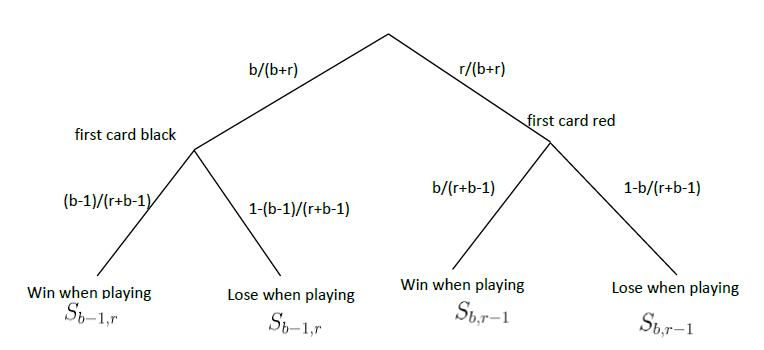
\includegraphics[width = 150mm]{last_problem.jpg}
\end{center}
\fi

\end{solution}
\eparts

\end{problem}
